\section{Evolução arquitetural}
O processo de escolha para a arquitetura utilizada foi iterativo, e foram analisados os pontos fracos e as vantagens de cada nova sugestão.

A primeira versão proposta baseava-se unicamente em microsserviços, responsáveis por toda a inteligência do projeto, o que a fazia interessante do ponto de vista da escalabilidade para um número muito grande de casas. Com uma arquitetura fundamentalmente desenvolvida assim, também é possível utilizar quantas tecnologias forem necessárias ou desejáveis para cada um dos serviços sem efeitos colaterais nos outros, ou seja, transparentemente. Por outro lado, cria-se grande uma complexidade na integração entre todos os serviços disponíveis, que pode ser gerenciada por técnicas conhecidas e também explicadas aqui, como a coreografia e a orquestração. No entanto, há um aumento do \textit{overhead} para a comunicação, e os serviços do Hedwig necessitam de um meio rápido e robusto, que implemente qualidade de serviço para padrões diferentes de mensagens. Foi proposto um \textit{gateway} para os serviços da nuvem, por onde passaria toda a comunicação com a casa. A inserção do \textit{gateway}, no entanto, cria um ponto único de falha.

\begin{figure}[H]
	\centering
	\caption{Primeira versão da arquitetura do projeto Hedwig}
  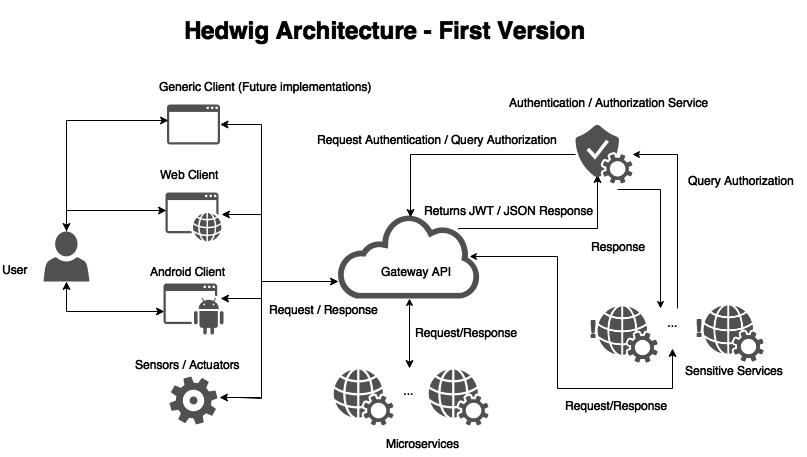
\includegraphics[width=0.8\textwidth]{arquiteturaV1}
\label{fig:arquiteturaV1}
\end{figure}

É possível observar que alguns microsserviços são classificados como sensitivos, os quais dependem de nova consulta ao serviço de autenticação e autorização para garantir a segurança. Esses serviços são todos aqueles responsáveis por tomar uma ação em relação à casa que envolva riscos. Os microsserviços não-sensitivos utilizam a autenticação já realizada pelo \textit{gateway} na chegada da requisição.

Quando uma requisição chega à nuvem, ela deve ser autenticada, e caso passe nos critérios de autenticação e autorização, é retornado um JWT (\textit{JSON Web Token}), necessário para os passos seguintes. O JWT é discutido aqui, na seção MARCAR SEÇÃO AQUI. % TODO marcar seção

De extrema importância, e não cobertos pela arquitetura anterior, são os requisitos de disponibilidade do projeto. Se o \textit{gateway} estiver inacessível em determinado momento, a casa não terá mais nenhuma forma de comunicação com os meios externos, mesmo para os serviços mais básicos. Para resolver este problema, foi proposta uma segunda versão, conforme ilustra a imagem seguinte.

\begin{figure}[H]
	\centering
	\caption{Segunda versão da arquitetura do projeto Hedwig}
  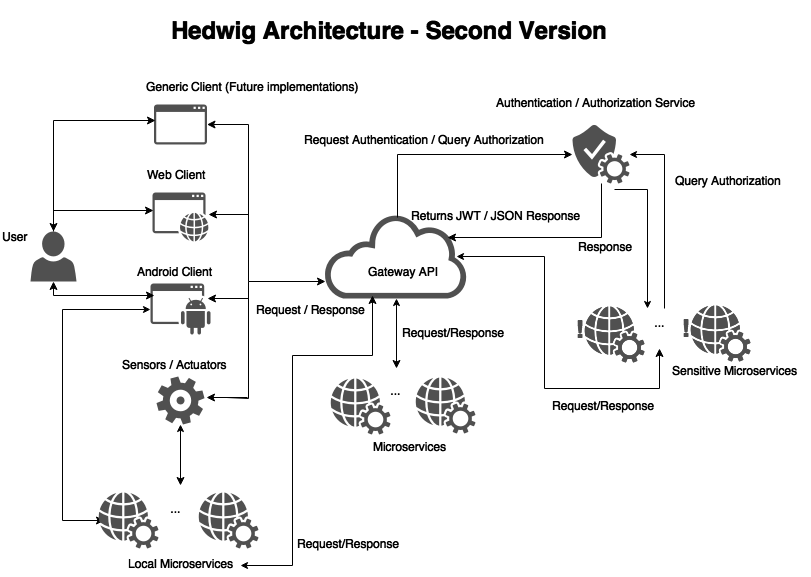
\includegraphics[width=0.8\textwidth]{arquiteturaV2}
\label{fig:arquiteturaV2}
\end{figure}

Nesta versão, serviços essenciais seriam duplicados dentro da casa, e, no caso de haver qualquer forma de impedimento na comunicação com a nuvem, esses serviços seriam responsáveis por controlar diretamente os atuadores desejados. Entretanto, cria-se mais uma complexidade ao manter serviços duplicados na casa, e, no caso destes serviços não estarem online no momento necessário, também não seriam alcançados requisitos mais fortes de disponibilidade. Contudo, é uma versão que chega mais próxima de obedecer às necessidades do projeto.

Essa arquitetura provê módulos sem inteligência, e todo o controle é feito pelo serviço correspondente. Ao mesmo tempo, essa escolha tem benefícios como a escalabilidade, a manutenção (já que é muito mais simples atualizar o software de um ponto único, sempre que necessário) e a facilidade para prover correções ou possíveis aumentos de funcionalidade. Porém, não ficaríamos livres, mais uma vez, do ponto único de falha. Outro ponto é que alguns módulos ficariam em lugares de difícil acesso, ou mesmo fora da casa, onde a comunicação poderia ser perdida ou ser intermitente. Assim, em caso de falha de comunicação, um atuador não receberia os sinais necessários do serviço, acarretando em sérios problemas de segurança. No caso de uma garagem, por exemplo, o portão permaneceria aberto indeterminadamente, ou poderia não ser aberto quando o morador chegasse em casa.

Assim, começamos o desenvolvimento de um modelo arquitetural modularizado, onde cada módulo teria inteligência para realizar as tarefas necessárias e, ao mesmo tempo, pode enviar dados à nuvem e ser avisado quando deve realizar uma tarefa. Além disso, no aspecto comercial, módulos inteiros poderiam ser vendidos, substituídos e aumentados.

A arquitetura escolhida faz uso de microsserviços no lado da nuvem, e, no lado da casa, os componentes de hardware passam a ser agrupados em módulos independentes, com responsabilidades bem estabelecidas, inteligência e autonomia para realizar todas as atividades necessárias, e com comunicação a um servidor local, que realizará, por último, a comunicação direta com os serviços não locais. Esse servidor se comunicaria com os módulos por meio de mensagens enviadas em tópicos, as quais seriam interpretadas e enviadas aos servidores remotos.

Em uma eventualidade de a comunicação entre o servidor local e a nuvem ser perdida, os aplicativos web ou \textit{mobile}, podem se comunicar diretamente com o servidor local da casa, para acessar uma quantidade mais restrita e essencial de ações - como, por exemplo, a liberação de acesso à casa. Nessa situação, o servidor local armazena as mensagens, que serão enviadas ao servidor remoto posteriormente. Essas mensagens, no caso, seriam de dados, advindas de sensores em módulos. Como não há urgência para o processamento de tais dados, os quais serão utilizados para análise de comportamento e Machine Learning, não há prejuízo com o eventual envio tardio. O único prejuízo em tal situação seria no caso de o usuário não estar conectado à sua rede local, situação na qual não seria possível visualizar por meio de aplicativo web ou \textit{mobile} informações sobre o status dos sensores e atuadores em seus módulos.

Além disso, no caso de perda de comunicação tanto com a nuvem como com o servidor local, os aplicativos poderão se comunicar diretamente com os módulos para terem acesso aos serviços de extrema importância.

Por ter sido escolhida, essa arquitetura será extensivamente detalhada e discutida aqui, com seus benefícios e limitações.
